\documentclass{standalone}
\usepackage{tikz}
\usetikzlibrary{positioning,shapes.geometric,arrows}
\begin{document}
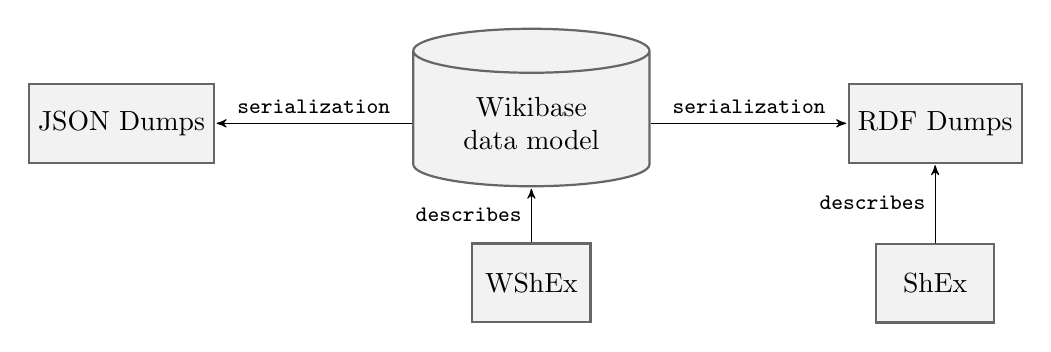
\begin{tikzpicture}[
        serialization/.style={
                rectangle,
                draw=black!60,
                fill=black!5,
                thick,
                minimum width=20mm,
                minimum height=10mm
            },
        schema/.style={
                rectangle,
                draw=black!60,
                fill=black!5,
                thick,
                minimum width=15mm,
                minimum height=10mm
            },
        db/.style={
                cylinder,
                draw=black!60,
                fill=black!5,
                thick,
                minimum width=30mm,
                minimum height = 20mm,
                shape border rotate=90,
                aspect=0.25,
                text width = 20mm,
                text centered
            },
        predicate/.style = {font=\footnotesize\ttfamily},
        >= stealth',
        shorten >= 0.5pt
    ]
    \node[db] (dataModel) {Wikibase data model};
    \node[serialization] (JSON) [left=2.5cm of dataModel] {JSON Dumps};
    \node[serialization] (RDF) [right=2.5cm of dataModel] {RDF Dumps};
    \node[schema] (ShEx) [below=1cm of RDF] {ShEx};
    \node[schema] (WShEx) [below=0.7cm of dataModel] {WShEx};

    \path[->] (dataModel.west) edge node[predicate,above] {serialization} (JSON.east);
    \path[->] (dataModel.east) edge node[predicate,above] {serialization} (RDF.west);
    \path[->] (ShEx.north) edge node[predicate,left] {describes} (RDF.south);
    \path[->] (WShEx.north) edge node[predicate,left] {describes} (dataModel.south);
\end{tikzpicture}
\end{document}